\scanpage{87}
% archive foliation: 86
par produit tensoriel des formes
[N.B. le produit tensoriel de deux formes
\deleted{symétriques, ou de} de même type de symétrie
est symétrique --- de deux types opposés
de symétrie est antisymétrique]. Bien
entendu, ils ne sont pas en général
bijectifs (mais du moins injectifs).

On a aussi
\[
\Phi^s(M'\times M'')\simeq\Phi^s(M')\times\Phi^s(M'')\times B(M',M'')
\]
où $B(M',M'')=\operatorname{Hom}(M'\otimes M'',\mathbf Q(\rho))$.

Ceci posé, on \deleted{\unsure{aura pour $d$}}\inserted{a dans}
$\Phi^s(M)$ un cône \inserted{convexe} fermé $\Phi^+(M)$.
\figure{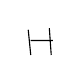
\begin{tikzpicture}[scale=.4]
\draw (0,0)--(-.08,.8) (0,.46)--(.7,.46) (.65,0)--(.59,.85);
\end{tikzpicture}}
On a les propriétés suivantes :

(i) $\Phi^+(M)$ a un intérieur non vide.

(ii) Un élément de $\Phi^+(M)$ est dans l'int. de $\Phi^+(M)$ ssi il est non dég.

\margin{formes $\in\Phi^+(M)$ sont dites pseudo-amples, celles
dans l'intérieur sont dites \uline{amples}}

(iii) Pour $M\longrightarrow N$, $\Phi^+(N)$ s'envoie dans $\Phi^{\unsure{s|+}}(M)$.

(iv) \deleted{\unsure{(iii)} \unsure{Pour}} Si $M\longrightarrow N$ injectif,
\deleted{$\Phi^+(\unsure{N|M})$} l'intérieur
de $\Phi^+(N)$ s'envoie dans l'intérieur
de $\Phi^+(M)$ (forme ample $\longrightarrow$ forme ample)
